\documentclass[a4paper]{article}
\usepackage[utf8]{inputenc}
\usepackage[natbib,sorting=none]{biblatex}
\usepackage{graphicx}
\usepackage{acronym}
\usepackage{indentfirst}
\usepackage[none]{hyphenat}
\usepackage{fancyhdr}
\usepackage{enumitem}
\usepackage{xcolor}

\addbibresource{references.bib}
\newcommand{\comment}[1]{\textbf{Comment: #1}}

\begin{document}
\begin{figure}[!h]
	\centering
	
\includegraphics[width=80mm]{images/poli-logo.png}
\end{figure}
\hfill
\begin{center}
    \fontsize{18px}{6mm}\selectfont \textsc{\textbf{Software Engineering II project}}
\end{center}
\begin{center}
    \fontsize{12px}{4mm}\selectfont \textsc{Academic Year: 2018/2019}
\end{center}
\hfill
\hfill
\begin{figure}[!h]
	\centering
	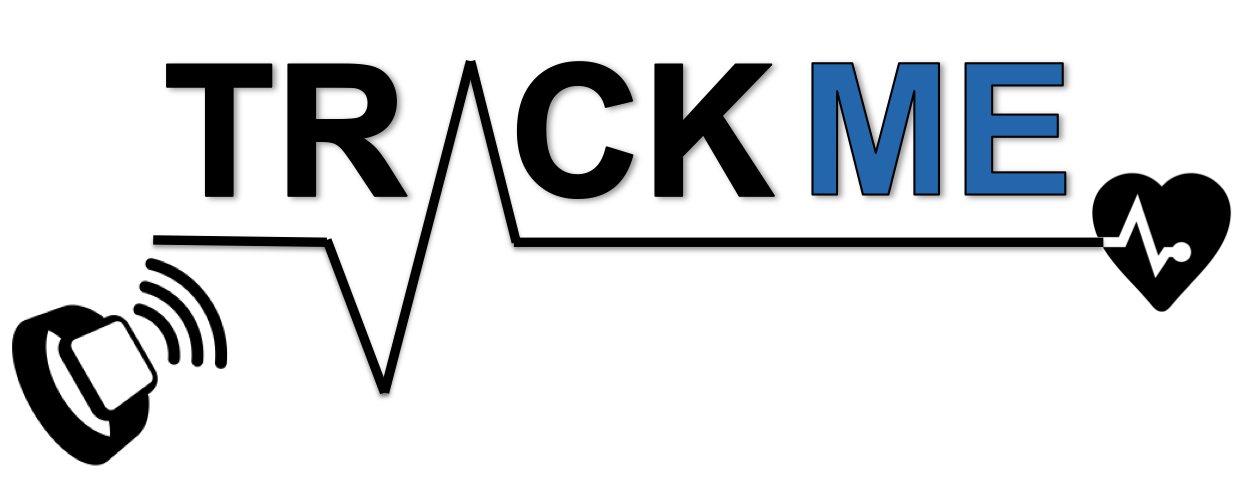
\includegraphics[width=120mm]{images/trackme-logo.png}
\end{figure}
\hfill
\hfill
\begin{center}
    \fontsize{22px}{8mm}\selectfont \textsc{\textbf{Requirement Analysis and\\ Specification Document}}
\end{center}
\begin{center}
    \fontsize{14px}{4mm}\selectfont \textsc{{Draft Version 0.1 - 11/10/2018}}
\end{center}
\hfill
\hfill
\begin{center}
\fontsize{14px}{4mm}\selectfont \textsc{\textit{Davide Rutigliano -  903616}}
\end{center}

\begin{center}
\fontsize{14px}{4mm}\selectfont \textsc{\textit{Claudio Ferrante - 903417\\}}
\end{center}

\begin{center}
\fontsize{14px}{4mm}\selectfont \textsc{\textit{Davide Matta - 903616}}
\end{center}
\pagenumbering{roman}
\tableofcontents
\newpage
\pagenumbering{arabic}
\section{Purpose and Scope}
This document is intended for presenting how all the features presented and designed in previous documents have been implemented \cite{dd}\cite{rasd}. In addition, the document be points out rationale for design choices for the adopted development frameworks.

This paper also contains a detailed description of the whole implementation both of client and server code and further testing following the \textit{I\&T plan}.

Finally, it contains all the installation and build instruction both for client and server, needed to run the code.

This document is intended for developers or anyone interested in the impleme-\newline ntation details of \textit{TrackMe}.

\section{Requirements and Functions}
This chapter is focused on highlighting requirements presented in previous documents, assuming the reader has previously read both Requirement and Design Document. In particular requirements implemented are from Data4Help and Track4Run services; AutomatedSos functionality instead has been not imple-\newline mented because not requested by the customer.

\section{Adopted Development Frameworks}

\subsection{Programming Language}
For both server and client side application the adopted language is Java: version 8 server-side, version 7 client-side; version 7 for mobile application is in order to support older OS version such as \textit{Android KitKat (4.0)}. The rationale for this choice is that Java is more suitable for large-scale application with respect to other programming languages. In addition it has a large number of libraries and frameworks and it is also supported by android, needed for the client application.

\paragraph{Pros:}

\begin{itemize}
    \item Object Oriented language
    \item Cross-Platform support
    \item Proprietary implementation of Persistence API
    \item Proprietary implementation of Authentication and Access Control
    \item Test-driven development
    \item Scalability
    \item High Performance
\end{itemize}

\paragraph{Cons:}
\begin{itemize}
    \item Code Verbosity
\end{itemize}

\subsection{Frameworks, Libraries and Others}

\paragraph{Server-Side Frameworks}
\begin{itemize}
    \item Spring Framework: this choice is an alternative to Java Enterprise Edition and Enterprise Java Bean based models. The main advantage of this framework is indeed that allows programmers to write less code and to focus on critical parts of the application instead of \textit{"simple and standard"} things. For instance, Spring Boot allows developers to create application with embedded web server such as Tomcat or Jetty with few lines of configuration without installing the web server itself. In addition, this framework also supports dependency injection and inversion of control. These latter features also allows developer to speed up and facilitate unit testing.
\end{itemize}

\paragraph{Client-Side Libraries}
In the Design Document we proposed Google for Map libraries, but since June 2018 Google Maps is not free anymore, we implemented our custom version of the map, using following libraries:
\begin{itemize}
    \item Osmdroid
    \item Osmbonuspack
    \item GraphView
\end{itemize}

\paragraph{NOTE:} In a production system it may be better to use Google Maps API to manage maps as their libraries are widely used and tested with respect to a custom map implementation.

Moreover, for STOMP protocol, we implemented our set of libraries in order to make it work because public libraries available online does not or does bad work.

\paragraph{Other Software}
\begin{itemize}
    \item MySQL Database as database system
\end{itemize}

\subsection{API}
\begin{itemize}
    \item Wear OS (Android Wear) API in order to make the mobile application communicate with an external devices such as a smartwatches.
\end{itemize}

\newpage
\section{Structure of the Code}
The application has been implemented following the design document, then structure of the code is almost the same presented into component and class diagrams, with little modifications skipped in the design document in order to not overload them.

Furthermore, the overall structure of both client and server application is organized in packages in order to improve reusability and maintainability of the code.

\subsection{Server Code Packages}
\begin{itemize}
\item \textbf{config:} spring configuration classes for security and web sockets
\item \textbf{constant}
\item \textbf{model:} contains two sub-packages, first spring entities used by repositories and second DTO classes related to entities
\item \textbf{repository:} spring crud repository classes
\item \textbf{service:} spring services, the business logic of the application
\item \textbf{controller:} spring controllers, handles communications between server logic and client presentation layer
\item \textbf{token:} contains spring security token authentication filter and token utilities
\end{itemize}

\subsection{Client Code Packages}
\begin{itemize}
\item[]
\end{itemize}

\newpage
\section{Testing}
Testing code is available within the project directory in "test" package.

\subsection{Server Side Testing}
Server-side code has been tested using the tools provided by Java with some additional libraries. In particular were used the JUnit to test the part that works in local without using external resources such as DBMS or network and Mockito, a popular mock framework which can be used in conjunction with JUnit.

\subsection{Client Side Testing}

\newpage
\section{Install Instructions}

\newpage
\section{Effort Spent}
    \begin{itemize}
        \item[-] \textbf{Davide Rutigliano: }
        
        \item[-] \textbf{Davide Matta: }
        
        \item[-] \textbf{Claudio Ferrante: }
    \end{itemize}
\end{document}